\documentclass[
    12pt,
    oneside,
    a4paper,
    english,
    brazil
]{abntex2}

\usepackage{lmodern}
\usepackage[T1]{fontenc}
\usepackage[utf8]{inputenc}
\usepackage{indentfirst}
\usepackage{color}
\usepackage{graphicx}
\usepackage{microtype}
\usepackage{amsfonts}
\usepackage{csquotes}

\usepackage{tikz}
\usetikzlibrary{positioning}

\usepackage{caption}

\usepackage[brazilian,hyperpageref]{backref}
\usepackage[alf]{abntex2cite}

\usepackage{macros}

\titulo{Previsão de séries temporais por meio de aprendizado de máquina}
\autor{Guilherme Chichanoski}
\local{Maringá}
\data{2018}
\orientador{Valéria Delisandra Feltrim}
\instituicao{Universidade Estadual de Maringá\\
Centro de Tecnologia --- Departamento de Informática\\
Bacharelado em Ciência da Computação}
\tipotrabalho{Trabalho de Conclusão de Curso}

\preambulo{Trabalho de Conclusão de Curso de Graduação apresentado ao
Departamento de Informática da Universidade Estadual de Maringá, como requisito
parcial para obtenção do grau de Bacharel em Ciência da Computação.}

\makeatletter
\hypersetup{
    pdftitle={\@title},
    pdfauthor={\@author},
    pdfsubject={\imprimirpreambulo},
    pdfcreator={LaTeX with abnTeX2},
    pdfkeywords={séries temporais}{arima}{aprendizado de máquina}{redes neurais},
    colorlinks=true,        % false: boxed links; true: colored links
    linkcolor=red,         % color of internal links
    citecolor=green,         % color of links to bibliography
    filecolor=magenta,      % color of file links
    urlcolor=blue,
    bookmarksdepth=4
}
\makeatother

\setlength{\parindent}{1.3cm}
\setlength{\parskip}{0.2cm}

\begin{document}

\frenchspacing

\imprimircapa{}

\imprimirfolhaderosto{}

\begin{resumo}
    % TODO: Resumo

    \textbf{Palavras-chave}: séries temporais, arima, aprendizado de máquina,
    redes neurais.
\end{resumo}

\begin{resumo}[Abstract]
    \begin{otherlanguage*}{english}
        % TODO: Abstract

        \textbf{Keywords}: time series, arima, machine learning, neural
        networks.
    \end{otherlanguage*}
\end{resumo}

\textual{}

\pdfbookmark[0]{\contentsname}{toc}
\tableofcontents*
\cleardoublepage{}

\chapter{Introdução}

Segundo \citeonline{wiley} prever é a tarefa de predizer valores futuros ou
eventos, é de grande importância para diversos setores incluindo governos e
industrias. Sendo parte crucial na tomada de decisão fica evidente a
necessidade de se realizar boas previsões. No entanto, essa tarefa muitas vezes
pode ser extremamente complexa, muitos autores e organizações já realizaram
previsões que se demonstraram erradas, como exemplo podemos citar o The New
York Times que previu em 1966 que em 2000 existiriam somente 220.000
computadores nos Estados Unidos.

Ainda conforme \citeonline{wiley} as previsões são classificadas como sendo de
curto, médio e longo prazo, sendo o prazo definido na frequência das
observações.  Quando denominada de curto é previsto somente poucas observações
a frente. Já previsões de médio prazo podem se estender por algumas observações
no futuro, enquanto períodos maiores serão chamados de longo prazo. Ainda
conforme o autor, predições de médio e longo prazo são mais difíceis e
suscetíveis a fatores externos.

% FIXME Acredito que deveria estar nos trabalhos relacionados
%Em \citeonline{giebel2011state} o autor realiza a predição da geração de
%energia eólica, a produção é dada em função da capacidade na região instalada,
%o vento, no entanto, é um elemento volátil e sendo assim existirá momentos
%quais o uso de outras fontes será necessária, contudo, é preciso ter certo
%conhecimento prévio, pois, o ligamento de uma usina como aquelas movidas a
%gasóleo podem levar até duas horas. Logo prever duas horas a frente pode ser
%crucial para garantir o abastecimento de energia a uma região, podendo
%impactar no cotidiano e economia de uma população.

Para a realização da previsão é necessário ter uma grande compreensão do que se
quer prever, sendo necessário organizar a informação de uma forma a evidenciar
a dependência dos dados com seus estados anteriores, para isso podemos
apresentar essas informações na forma de uma série temporal e a partir dessa
realizar medições e produzir modelos, que deverão ser capazes de expressar
matematicamente o comportamento da série em função de suas observações
anteriores, permitindo obter predições de estados futuros.

% FIXME: Tá esquisito
As séries temporais, segundo \citeonline{wiley} são compostas de observações
sequenciais ao longo do tempo, como exemplo, podemos observar a série na
\autoref{serie0}, que foi gerada utilizando um processo de caminhada aleatória.
Sendo essas observações separadas unicamente pelo tempo pode-se obter os dados
em diferentes intervalos, como observações diárias, semanais ou ainda anuais.
Conforme \citeonline{ehlers} devido a caraterística estocástica uma observação
é definida por ser dada em função de suas antecessoras.

\begin{figure}[ht]
    \centering
    \caption{Série gerada para exemplo}\label{serie0}
    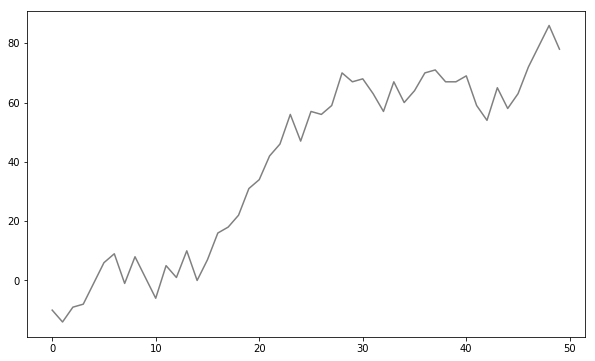
\includegraphics[width=.6\linewidth]{images/serie_exemplo.png}
    \source{Elaborado pelo autor}
\end{figure}

Considerando então que a série apresentará comportamento estocástico podemos
propor modelos que serão capazes de aproximar o comportamento da série, e os
modelos comumente utilizados nessa tarefa são aqueles probabilísticos, mais
especificamente o proposto por \citeonline{box} conhecido por ARIMA\@. Em
contrapartida podemos apresentar modelos utilizando aprendizado de máquina para
expressar essas séries que vem se apresentando como uma alternativa poderosa em
muitas aplicações.

Com o constante interesse na aplicação e identificação das capacidades de
técnicas de aprendizado é evidente a importância de observar como esse
modelo se compara com aqueles estatísticos. Como forma de identificar essa
diferença e buscar compreender as técnicas esse trabalho realizou a previsão de
uma série de característica econômica utilizando ambas metodologias.

% TODO: Introduzir modelos ARIMA com exemplos de artigos

% FIXME Mais adequado na parte de trabalhos relacionados
%vez mais notórias pelos bons resultados que oferecem. \citeonline{artigoEx3}
%Em contrapartida, técnicas de aprendizado de máquinas estão se tornando cada
%aplicou métodos de aprendizado de máquina possibilitando a previsão com bons
%resultados.  Pelo fato dos modelos estatísticos fornecerem resultados
%satisfatórios para predições e estarem bem difundidos na comunidade acadêmica,
%é comum que trabalhos como \citeonline{artigoEx4} compare os resultados
%obtidos a partir de aprendizado de máquina com modelos de abordagem
%estatísticas. Para modelos de aprendizado se destaca aqueles com uso de redes
%neurais artificiais por serem capazes de obter bons resultados conforme
%analisado por \citeonline{zhang}, o autor ainda apresenta outros exemplos
%quais os autores obtiveram resultados superiores ao método estatístico.

Esta monografia se organiza da seguinte forma, na \autoref{chap:fundTeor} será
apresentada a definição da atividade de previsão seguido dos principais métodos
de previsão de séries temporais empregadas, sendo o primeiro, ARIMA, com
abordagem estatística e o segundo usando com base em métodos de aprendizado de
máquina, sendo especificamente descrito as redes neurais artificiais de
múltiplas camadas. Após apresentado os métodos, no \autoref{chap:desenv}
conforme objetivos estabelecidos serão propostos dois modelos, um utilizando o
modelo probabilístico e o outro tendo base o modelo de inspiração biológica.
Com base nos modelos obtidos serão apresentados os resultados no
\autoref{chap:result} e finalizando com a discussão dos resultados obtidos no
\autoref{chap:concl}.

\chapter{Fundamentação teórica}\label{chap:fundTeor}

\section{Previsão}
Segundo \citeonline{wiley} podemos separar o processo de previsão em diversas
atividades, dispostas a seguir:

\begin{enumerate}
    \item Definição do problema\\
        Envolve definir e entender a tarefa de previsão a ser realizada,
        considerando o prazo a ser previsto e definindo os dados necessários.
    \item Coleta dos dados\\
        Conforme o problema definido na etapa anterior ocorrerá nessa atividade
        a coleta dos dados necessários.
    \item Análise dos dados\\
        Atividade de alta importância para a seleção do modelo mais adequado,
        nessa etapa é utilizada de observações gráficas e extração de
        características para identificar padrões que corroborem na escolha dos
        parâmetros. Ainda ocorrerá a identificação de observações problemáticas
        e aplicadas as devidas correções.
    \item Seleção e verificação do modelo\\
        Conforme análise será selecionado o modelo, analisando também o
        comportamento com os dados fornecidos. Como método de verificação será
        utilizado métricas que favoreçam a comparação.
    \item Avaliação do modelo\\
        Etapa para avaliar como o modelo se comportará com novos dados,
        normalmente é realizado com observações excluídas dos dados utilizados
        nas etapas anteriores, porem a parte separada terá somente esta
        finalidade.
    \item Publicação do modelo\\
        Com o modelo devidamente selecionado e avaliado é instalado em ambiente
        de produção, tendo que observar as alterações necessárias para que
        novos dados sejam inseridos corretamente.
    \item Monitoramento do desempenho do modelo\\
        Deve-se continuamente avaliar como o modelo aplicado se comporta em
        relação ao ambiente, já que o ambiente é algo volátil.
\end{enumerate}

As atividades normalmente são empregadas em ordem semelhante a exposta. Vale-se
ainda observar que após a tarefa de avaliação, se essa resultar em um valor
insatisfatório, deve-se retornar a fase anterior e refeita a avaliação até que
um modelo que obedeça às especificações seja encontrado.

\section{Séries temporais}

Como já disposto anteriormente, séries temporais são observações sucessivas ao
longo do tempo. Retomamos ainda que essas séries se caracterizam pelo fato de
suas observações serem dependentes das observações anteriores. Demonstram
características como tendência e sazonalidade, sendo que a primeira capaz de
conferir a série um lento comportamento que pode levar a observações futuras
com valores menores ou maiores e a segunda característica confere a ela padrão
que pode vir a apresentar ciclos dados em função do tempo, comumente tomando
períodos semanais, mensais ou anuais.

Uma série é descrita matematicamente pelo conjunto $\{X(t): t \in T\}$, podendo
ser $t$ um tempo contínuo ou discreto, sendo continuo quando se possui as
observações de todo $t$ em $T$, sendo este dado como $T \subseteq
\mathbb{R}^{+}$ e discreto quando entre uma observação e outra existe um
intervalo igual de tempo, normalmente dado na forma de uma sequência, $T = \{1,
2, \ldots, n\}$, sendo $n$ o número de leituras.

Segundo \citeonline{ehlers} uma série temporal classicamente é decomposta
seguindo a \autoref{eq:timeseries}, sendo $t$ usado para denotar o tempo, $T$
nos fornece a tendência, $C$ a sazonalidade, já $R$ é a componente aleatória e
caracterizada por possuir média zero, denotada como ruído branco.

\begin{equation}
    \label{eq:timeseries}
    X_t = T_t + C_t + R_t
\end{equation}

\subsection{Série estacionária}

Um conceito importante durante a analise de séries é o caráter estacionário, e
segundo \citeonline{ehlers} definimos uma série estritamente estacionária por
possuir a distribuição de probabilidade conjunta de $X(t_1), \ldots, X(t_k)$
igual de $X(t_1 + \tau), \ldots, X(t_k + \tau)$.

Ainda segundo \citeonline{ehlers} a definição estrita dada é dificilmente
aplicada, então usualmente é aplicada a definição de fracamente estacionaria,
definindo então com base no critério de possuir função média constante.
Portanto, ao decorrer desse trabalho quando tomarmos uma série como
estacionária estamos concluindo isto pelo conceito de fracamente estacionária.
Em termos matemáticos podemos utilizar a \autoref{eq:westacionaria} para
definir que variância de um elemento da série deve ser semelhante a média.

\begin{equation}
    \label{eq:westacionaria}
    E(z_t) = \mu_t = \mu
\end{equation}

% FIXME Dada em função de que??
Em outras palavras, o deslocamento da origem do tempo $t$ por uma quantidade
$\tau$ não exerce efeito na distribuição conjunta da série, assim o valor
esperado para a série em determinado momento não será dada em função do tempo.

%TODO Adicionar referência ao Livro Time Series by exmples

%TODO Adicionar referência ao teste de Dockey Fuller


A \autoref{fig:co2diff} é um exemplo de série estacionária encontrada ao
aplicar o processo de diferenciação na série apresentada na \autoref{fig:co2},
este processo está descrito na \autoref{sec:diff}. Segundo
\citeonline{tsExample} embora exista testes como o de Dikey Fuller descrito em
\citeonline{dickey} para a prova de estacionáriedade, é suficiente a observação
gráfica da série.

\subsection{Tendência}

Segundo \citeonline{ehlers} não existe uma definição exata de tendência, mas
normalmente é associado ao comportamento de mudança das observações ao longo de
um vasto período. Uma série com tendência pode ser descrita como uma função
apresentada na \autoref{eq:tendencia}, $\alpha$ e $\beta$ coeficientes e
$\epsilon_t$ o erro. Sendo que $\beta$ define a taxa de crescimento da série,
assim podemos entender $\beta$ da forma $\beta = x_t - x_{t-1}$.

\begin{equation}
    \label{eq:tendencia} X_t = \alpha + \beta_t + \epsilon_t
\end{equation}

Este entendimento de série com tendencia segundo \citeonline{ehlers} já permite
encontrar uma função polinomial que represente a série, no caso esta toma a
forma da \autoref{eq:tendenciaSerie}.

\begin{equation}
    \label{eq:tendenciaSerie}
    X_t = \beta_0 + \beta_1t + \beta_2t^2 + \cdots + \beta_{p}t^p + \epsilon_t
\end{equation}

Para exemplificar uma série temporal real que apresente tendência e
sazonalidade podemos apresentar o gráfico na \autoref{fig:co2}, este apresenta
a mudança na concentração de $CO_2$ na atmosfera, no caso esta é uma série de
característica natural, é fácil notar a tendência de crescimento e sua
sazonalidade de periodicidade anual.

\begin{figure}
    \centering
    \caption{Leituras de $CO_2$ na atmosfera.}\label{fig:co2}
    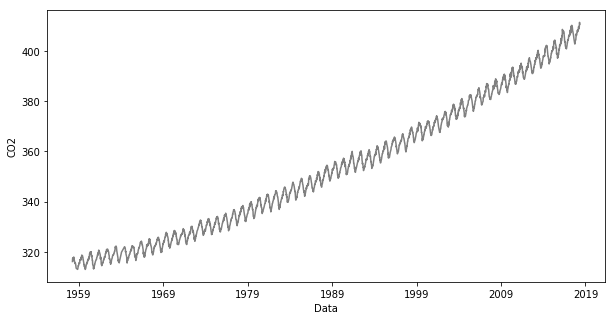
\includegraphics[width=.6\linewidth]{images/co2.png}
    \source{\citeonline{co2data}}
\end{figure}

\subsubsection{Filtros}

Em algumas séries a tendência pode não estar evidente devido à flutuações, por
conta disso pode vir a ser necessário a aplicação de filtros que tem como
objetivo obter uma série suavizada que possibilite observar a tendência, um
desses filtros é apresentado na \autoref{eq:filtro}\cite{ehlers}.

\begin{equation}
    \label{eq:filtro}
    y_t = \sum_{j = -q}^{s}{a_{j}x_{t+j}}
\end{equation}

Na \autoref{eq:filtro} $a_j$ é um coeficiente a ser aplicada a cada termo da
soma de forma a aplicar um peso a este, sendo observado que $\sum{a_j} = 1$.
Podemos obter no caso mais simples $a_j = \frac{1}{2q + 1}$ e teremos $y_j$
conforme a \autoref{eq:yjfiltro}.

\begin{equation}
    \label{eq:yjfiltro}
    y_t = \frac{1}{2q + 1}\sum_{j=-q}^{q}{x_{t+j}}
\end{equation}

A \autoref{eq:yjfiltro} é conhecida por fornecer o cálculo das médias móveis. A
aplicação do filtro de médias móveis na série das leituras de $CO_2$ resulta na
\autoref{fig:co2filtrado}, que evidencia de forma independente a tendência da
série após removido a sazonalidade.

\begin{figure}
    \centering
    \caption{Leituras de $CO_2$ filtrada utilizando médias móveis com $q$ igual
        a $52$, devido à sazonalidade ser anual, ou seja, $52$
        semanas.}\label{fig:co2filtrado}
    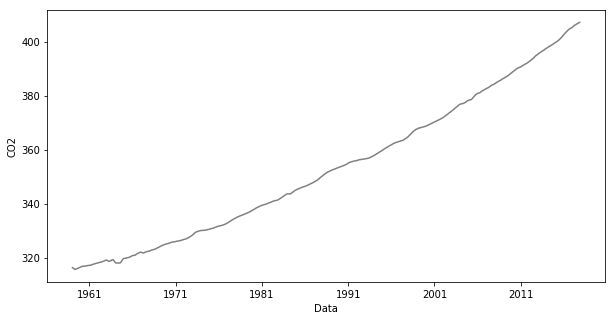
\includegraphics[width=.6\linewidth]{images/co2_filtered.png}
    \source{Elaborado pelo próprio autor a partir de \citeonline{co2data}}
\end{figure}

\subsubsection{Diferenciação}\label{sec:diff}

Outra tarefa a ser observada em relação ao entendimento de tendência é a forma
qual é removida, para sua remoção o método mais simples para tal é fazer a
subtração do valor observado com o seu antecessor, da forma como descrito na
\autoref{eq:diferenciacao}, normalmente uma única diferenciação é suficiente
porem em séries com componente sazonal podem vir a ser necessárias mais de uma
em um \textit{lag} diferente.

\begin{equation}
    \label{eq:diferenciacao}
    y_t = x_t - x_{t-1}
\end{equation}

Para dar um exemplo de diferenciação volto a série das leituras do $CO_2$ e
agora realizando uma diferenciação, o resultado é visto na
\autoref{fig:co2diff}, especificamente neste exemplo percebemos que a série se
aproximou de uma série com função média constante, dando evidência a componente
sazonal.

\begin{figure}
    \centering
    \caption{Série da leitura do $CO_2$ na atmosfera com uma
        diferenciação}\label{fig:co2diff}
    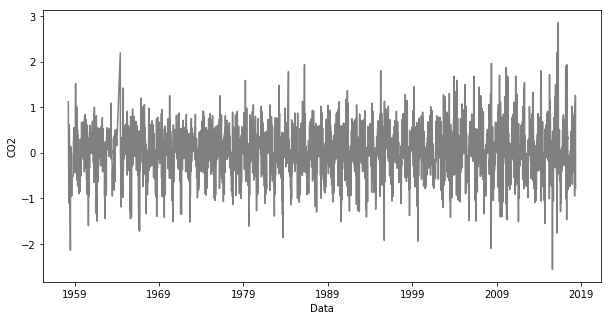
\includegraphics[width=.6\linewidth]{images/co2_diff.png}
    \source{Elaborado pelo autor a partir de \citeonline{co2data}}
\end{figure}

\subsection{Sazonalidade}

Conforme definido por \citeonline{ehlers} sazonalidade caracteriza repetições
de comportamento de uma série em um período $s$ de tempo. Normalmente é
facilmente observado na representação gráfica da série.

\section{Modelos probabilísticos}

Como já disposto, as séries temporais podem ser previstas utilizando de modelos
estatísticos, isso segundo \citeonline{ehlers} ocorre devido ao seu caráter
estocástico por conta de cada observação possuir correlação com as observações
imediatamente antecessoras diferentemente de séries determinísticas, quais tem
seu estado definido por uma função matemática ou um sistema onde a saída só é
dependente das entradas atuais.

O modelo comumente utilizado para essa tarefa é o ARIMA, descrito por
\citeonline{box}, caracteriza a série em três parâmetros $(p,d,q)$, sendo cada
um associado a um processo, sendo $p$ associado a processos auto-regressivos,
$r$ a processos integrativos e $q$ a de médias móveis.

Para encontrarmos esses parâmetros \citeonline{box} descreveu alguns processos,
entre eles a analise da função de autocorrelação.

\subsection{Função de autocorrelação}\label{sec:corre}

Durante a parametrização precisaremos identificar o comportamento da série, uma
ferramenta para isso é a função de autocorrelação, com base na correlação entre
duas séries $X$ e $Y$, podemos obter a correlação de uma série com defasagem
$k$, sendo essa defasagem a distância entre o valor analisado $X_t$ a
observação $X_{t-k}$.

Assim podemos obter a função de autocorrelação para uma série de 100 elementos
ao considerar que a série $X$ é os 99 primeiros elementos e $Y$ os 99 últimos
elementos. Assim a função de autocorrelação será dada segundo
\autoref{eq:autocorrelacao}.

\begin{equation}
    \label{eq:autocorrelacao}
    r_k = \frac{\sum_{t=1}^{n-k}{(x_t - \overline{x})(x_{t+k} -
    \overline{x})}}{\sum_{t=1}^{n}{(x_t - \overline{x})^2}}
\end{equation}

Segundo \citeonline{ehlers} a função de autocorrelação quando plotada para os
$k$-ésimos primeiros coeficientes é chamado de correlograma e este é uma
ferramenta importante para as análises, como exemplo pode ser visto a
\autoref{fig:correlogramaCo2} na qual é disposto as 25 primeiras defasagens das
leituras de concentração de $CO_2$ na atmosfera, ainda segundo
\citeonline{ehlers} temos de definir ao correlograma o seu intervalo de
confiança, com o qual podemos considerar tudo que esteja acima desse como uma
correlação que deve ser analisada e abaixo desse limite será desconsiderada,
assim se todos as correlações estarem abaixo desse limite podemos considerar a
série como um ruído branco, para encontrar esse intervalo \citeonline{ehlers}
recomenda utilizar a seguinte equação $\pm{}1,96/\sqrt{n}$, sendo $n$ o número
de observações da série.

\begin{figure}
    \centering
    \caption{Gráfico da função de autocorrelação das leituras de
        $CO_2$}\label{fig:correlogramaCo2}
    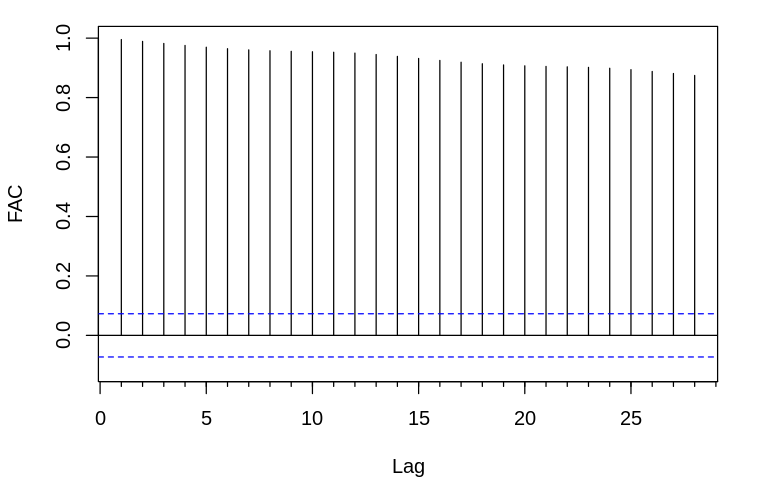
\includegraphics[width=.6\linewidth]{images/acf_co2.png}
    \source{Elaborado pelo autor a partir de \citeonline{co2data}}
\end{figure}

Pela \autoref{fig:correlogramaCo2} podemos concluir que as leituras do $CO_2$
apresentam uma tendência, e ainda por apresentar todos valores positivos
podemos afirmar que crescerá ao longo do tempo. Como a série possui tendência
temos de fazer uma diferenciação, como disposto na \autoref{sec:diff}, para
remoção dessa componente, vemos a série após essa diferenciação na
\autoref{fig:co2diff} e o correlograma após a diferenciação pode ser visto na
\autoref{fig:acfco2diff}, nesse novo gráfico é percebido que a componente da
tendência foi realmente removida após uma diferenciação, tornando visível a
componente sazonal, vemos isso pela alternância das correlações observadas no
correlograma.

\begin{figure}
    \centering
    \caption{Gráfico de função de autocorrelação da diferenciação da série de
        $CO_2$}\label{fig:acfco2diff}
    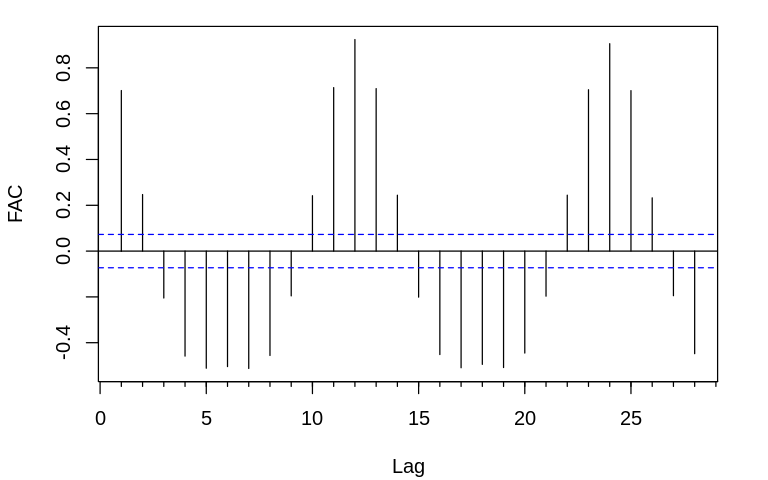
\includegraphics[width=.6\linewidth]{images/acf_co2_diff.png}
    \source{Elaborado pelo autor a partir de \citeonline{co2data}}
\end{figure}

% TODO: Citar as seções nas quais o correlograma é apresentada em outros
%cenários

\subsection{ARIMA}

O modelo ARIMA já introduzido na seção anterior possui três parâmetros
essenciais $(p,q,d)$ sendo $p$ repensável por definir o numero de observações
considerados no processo auto regressivo, $q$ o numero de diferenciações
necessárias para a remoção da tendencia e $d$ o numero de termos no processo de
medias móveis.

\subsubsection{AR -- Processo auto regressivo}

% TODO Melhor descrição da forma que é encontrado os coeficientes e a
% utilização do ACF e PACF para identificação do p

Segundo \citeonline{ehlers} um processo $X_t$ é chamado auto regressivo de
ordem $p$, ou $AR(p)$, quando temos $X_t$ dado segundo a
\autoref{eq:aregressivo}.

\begin{equation}
    \label{eq:aregressivo}
    X_t = \alpha_1X_{t-1}+\epsilon_t
\end{equation}

Como observado na \autoref{eq:aregressivo} é um modelo útil se for razoável
assumir que o valor atual depende somente de seus antecessores imediatos mais
um erro aleatório.

\subsubsection{MA -- Processo de médias móveis}

% TODO Melhor descrição da forma que é encontrado os coeficientes e a
% utilização do ACF e PACF para identificação do q

Segundo \citeonline{timeseriesExample} o processo de médias móveis é dado como
a média dos termos passados e correntes e pode ser descrito matematicamente
segunda a \autoref{eq:pmediasmoveis}.

\begin{equation}
    \label{eq:pmediasmoveis}
    X_t = \epsilon_t - \theta_1\epsilon_{t-1} - \theta_2\epsilon_{t-2} - \theta_{q}\epsilon_{t-q}
\end{equation}

Onde os valores de $\theta$ serão dados após análise da série.

\subsubsection{ARMA -- Modelo misto}

Combinando o processo AR e MA podemos obter um modelo extremamente útil para
descrever séries temporais. E a união dos modelos pode ser expressa pela
\autoref{eq:arma}.

%\begin{equation}
%    \label{eq:arma}
%    X_t = 

\subsubsection{Integração}

Em séries não estacionarias, segundo a definição dada na
\autoref{sec:estacionaria}, é necessário a transformação em uma série
estacionaria, isso pode ser simplesmente realizado utilizando o método descrito
na \autoref{sec:diferenciacao}, assim podemos aplicar de forma adequada o
procedimento de \citeonline{box} para produzir um modelo probabilístico que
poderá ser utilizado na atividade de previsão da série.

% TODO Referencias??
Normalmente uma diferenciação é suficiente para remover a tendencia de uma
série e a transformar em uma série estacionária, entretanto em séries que
apresentem a componente sazonal pode vir a ser necessária a aplicação de duas
ou mais diferenciações e em casos da aplicação de modelos SARIMA essa
diferenciação é aplicada com uma intervalo $l$, com esse valor sendo dado pela
sazonalidade da série.

\section{Aprendizado de Máquina}

Segundo \citeonline{machineLearning} aprendizado de máquina é descrito como a
habilidade de algorítimos reconhecer padrões em um conjunto de dados.

Esses padrões a serem encontrados permitirão que tarefas como as seguintes
seja, realizadas:
\begin{itemize}
    \item Classificação\\
        É a tarefa de mapear uma entrada a uma \textit{tag}, como no exemplo na
        classificação dos números, apresentada no início da seção. Podemos
        encontrar ainda exemplos do uso de aprendizado de máquina para
        classificação em diversos outros trabalhos, como
        \citeonline{artigoClassificacao} que utilizou redes neurais artificiais
        para realizar a classificação de imagens.
    \item Regressão\\
        Já a tarefa de regressão é aplicada quando precisamos mapear um
        conjunto de valores a uma saída em $ \mathbb{R} $,
        \citeonline{regressao} utilizou redes neurais artificiais para
        encontrar um modelo que permitisse a previsão da demanda de uso de
        energia elétrica, mapeando o carga atual e informações climáticas a
        carga futura.
\end{itemize}

Um exemplo de uso de aprendizado de máquina é a identificação de caracteres
numéricos escritos a mão, esse exemplo é apresentado por
\citeonline{machineLearning} e o descreve como um problema de classificação no
qual uma imagem de dimensões $28 \times 28$ pixeis é dada como entrada em um
algorítimo e este deve atribuir uma classificação que descreve qual o número
que a figura representa, um conjunto de exemplo dessas imagens pode ser visto
na \autoref{fig:numeroClassi}.

\begin{figure}
    \centering
    \caption{Exemplo de entrada para o algorítimo de
        classificação}\label{fig:numeroClassi}
    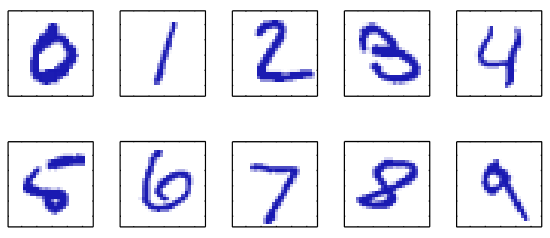
\includegraphics[width=.6\linewidth]{images/numeroClassificacao.png}
    \source{\citeonline{machineLearning}}
\end{figure}

\subsection{Redes Neurais artificiais}

Segundo \citeonline{haykin} a pesquisa em redes neurais artificiais é motivada
pelo entendimento que o cérebro humano realiza o processamento de uma forma
completamente diferente dos computadores convencionais. Essa forma de realizar
o processamento realizado pelo cérebro é altamente complexa, não linear e
altamente paralela. A unidade de processamento e organização básica de um
cérebro são os neurônios, o autor ainda lhe confere superior capacidade na
realização de tarefas como reconhecimento de padrões do que os computadores
digitais.

Os animais já nascem com o cérebro possuindo certa estruturas que estes vão
precisar durante sua vida, porem este é concebido ainda de maneira muito
plastica, ou seja, possuindo ainda a capacidade de na fase de aprendizado ser
capaz de se adaptar ao contexto em que vai se desenvolver. Este mesmo conceito
de plasticidade também será utilizado para a modelagem de redes neurais
artificiais~\cite{haykin}.

\subsubsection{\textit{Perceptron}}

Como já colocado, as redes neurais possuem o neurônio como elemento de
processamento, este em redes artificiais associamos ao \textit{perceptron},
descrito primeiramente por Rosenblatt em 1958, e tem sua função definida em
\autoref{eq:perceptron} sendo dado como a soma ponderada por $w_i$ das
entradas, $x_i$.

\begin{equation}
    \label{eq:perceptron}
    v = \sum_{i=1}^{m}{w_i + b}
\end{equation}

% TODO: Algorítimo
% TODO: MLP
% TODO: Back Propaggation
% TODO: Descida de Gradiente
% TODO: - Adam

\subsubsection{MLP}

\subsubsection{Adam}

\chapter{Desenvolvimento}\label{chap:desev}

Para demonstrar e avaliar a capacidade de os métodos de previsão apresentados
neste trabalho, foi selecionada uma série temporal qual consta as vendas
diárias de uma rede de farmácias germânica, os dados foram obtidos
\textit{online}\footnote{Kaggle
    \url{https://www.kaggle.com/c/rossmann-store-sales}}.

Foram realizadas algumas etapas de pré processamento dos dados antes de
obtermos a série temporal efetivamente utilizada para a previsão.
Primeiramente foi necessária a seleção de uma loja aleatoriamente, já que o
conjunto de dados obtidos nos traz dados das diversas lojas que compõe a rede.
Foi selecionada então de forma aleatória a loja de ID 67. Após foi então obtida
uma série temporal multivariada, entretanto, a proposta deste trabalho é a
avaliação de previsões em séries uni variadas, ou seja, embora o conjunto de
entrada possua mais informação que aquelas que serão utilizadas para previsão,
estas serão descartadas. Logo a série será composta somente da quantidade
diária de vendas realizadas. O gráfico que apresenta a série a ser encontrado o
modelo é vista na \autoref{fig:serieRossman}.

\begin{figure}[ht]
    \centering
    \caption{Gráfico de observações das vendas diárias}\label{fig:serieRossman}
    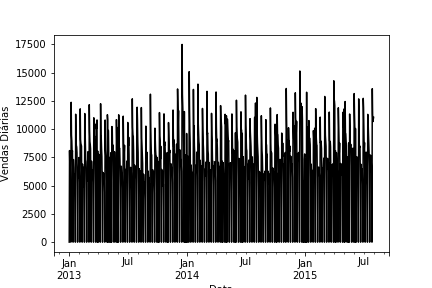
\includegraphics[width=.6\textwidth]{images/graficoRossman.png}
    \source{Elaborado pelo autor}
\end{figure}

\begin{figure}[ht]
    \centering
    \caption{Gráfico contendo 3 semanas de observações para visualização do
        comportamento semanal da série}\label{fig:serieRossmanSemana}
    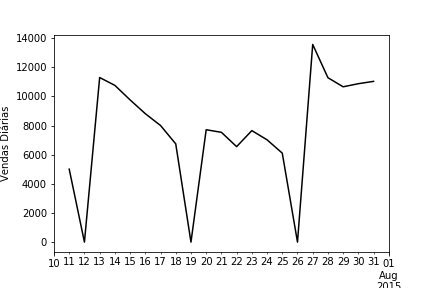
\includegraphics[width=.6\textwidth]{images/graficoRossmanSemana.png}
    \source{Elaborado pelo autor}
\end{figure}

Observamos na \autoref{fig:serieRossman} a existência de valores que podem ser
descritas como \textit{outliers}, isto é, são leituras que estão fora do padrão
esperado, isso ocorre devido às observações serem diárias e a rede de farmácia
não possuir expediente aos domingos, pode ser visto de forma mais clara na
\autoref{fig:serieRossmanSemana}, nesses dias as leituras aparecerão zeradas e
assim gerando uma série que embora com maior número de observações possuirá
instabilidade, que aumenta consideravelmente a complexidade do modelo, para
evitar esse problema foi realizada a conversão para observações semanais,
somando a quantidade de vendas realizada em uma semana em um único valor, essa
nova série é apresentada na \autoref{fig:serieRossmanSemanal}.

\begin{figure}[ht]
    \centering
    \caption{Gráfico de observações semanais de
        vendas}\label{fig:serieRossmanSemanal}
    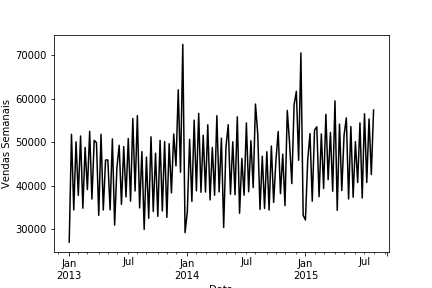
\includegraphics[width=.6\textwidth]{images/graficoRossmanSemanal.png}
    \source{Elaborado pelo autor}
\end{figure}

\section{Análise da série}

Para continuarmos com a parametrização dos modelos que serão avaliados temos de
ter uma boa compreensão do comportamento da série, para isso são aplicadas
algumas ferramentas apresentados como o correlograma descrito na
\autoref{sec:corre}.

Em primeira analise observamos na \autoref{fig:serieRossmanSemanal} que em dois
momentos a série apresenta máximos locais, observado de forma detalhada na
\autoref{fig:rossmanFimAno}.

\begin{figure}
    \centering
    \caption{Gráfico do comportamento da série no fim do
        ano}\label{fig:rossmanFimAno}
    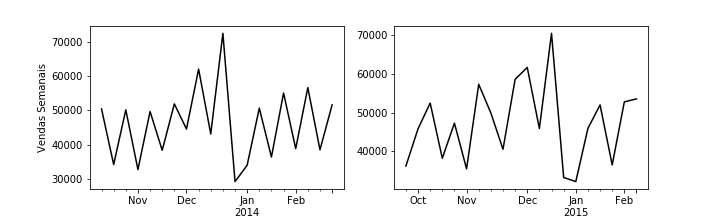
\includegraphics[width=.8\textwidth]{images/graficoRossmanFimAno.png}
    \source{Elaborado pelo autor}
\end{figure}

O conjunto de dados utilizado, ainda nos trás outras informações, como se houve
promoção naquele dia ou se foi feriado. Se considerarmos essas informações
podemos compreender algumas flutuações que ocorrem na série, por exemplo se
observarmos a \autoref{fig:rossmanPromo} vemos que os maiores volumes de venda
tendem a ocorrer nos dias de promoção.

% TODO: Gerar essa imagem
\begin{figure}
    \centering
    \caption{Observações marcados conforme ocorrência de promoções}
    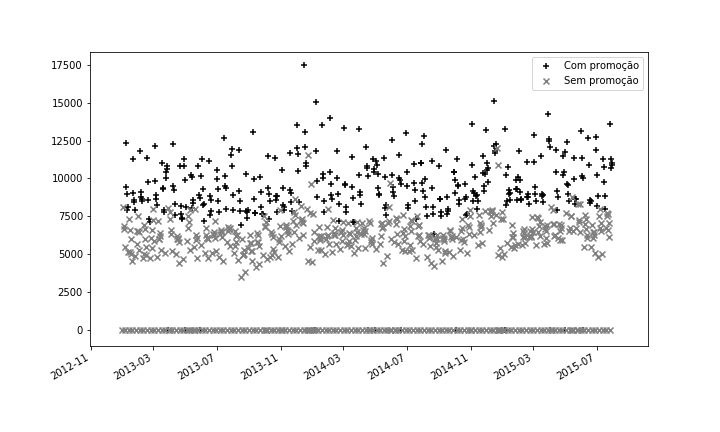
\includegraphics[width=.7\textwidth]{images/graficoRossmanPromo.png}
    \source{Elaborado pelo autor}
\end{figure}

Aplicando então a função de autocorrelação apresentada anteriormente obteremos
informações para a parametrização do modelo, utilizando a série com frequência
semanal apresentado na \autoref{fig:serieRossmanSemanal} teremos a seguinte
\autoref{fig:acfRossmanSemanl}.

% \begin{figure}
%     \centering
%     \caption{Função de Autocorrelação aplicada a série}
%     \includegraphics[width=.7\textwidth]{images/graficoAcfSemanal.png}
%     \source{Elaborado pelo autor}
% \end{figure}

\section{Aprendizado de máquina}

Diferentemente do ARIMA, redes neurais artificiais não foram elaboradas com a
visão na aplicação de previsão de séries temporais, na verdade seu uso é muito
mais abrangente que este, no entanto, se considerarmos o problema de previsão
de redes neurais como um problema de regressão poderemos modelar a rede neural
para que a saída desta seja a próxima observação da série.

A entrada da rede neural foi estabelecida como duas observações no passado,
porem poderia ser utilizado mais, mas para manter o modelo parcimonioso foi
mantido assim.

Na etapa de escolha dos parâmetros foi utilizado busca em grade com validação
cruzada, com \textit{fold} de tamanho cinco. Os parâmetros testados estão
apresentas na \autoref{tab:grid}, para validação do modelo foi calculado o MAPE
e então selecionado aquele que melhor representou a série.

\begin{table}
    \centering
    \caption{Parâmetros testados na busca em grade}\label{tab:grid}
    \begin{tabular}{ l r }
        \toprule
        Parâmetros                      & Valores testados\\
        \midrule
        Número de camadas escondidas    & [1, 2, 3, 4]\\
        Número de neurônios por camadas & [2, 4, \ldots, 100]\\
        Função de ativação              & [relu, tanh]\\
        Número de épocas                & [500, 1000, 1500]\\
        Otimizador                      & [adam, sgd]\\
        \bottomrule
    \end{tabular}
    \source{Elaborado pelo autor}
\end{table}

Após execução, o resultado da busca em grade retornou que a melhor escolha a
utilização de somente uma camada escondida com 12 neurônios, alem disso a
função de ativação ficou estabelecida como a relu, com otimização usando adam.
A arquitetura da rede neural resultante é demonstrada na
\autoref{fig:redeNeural}.

\begin{figure}
    \centering
    \caption{Representação gráfica da rede neural artificial utilizada para
        avaliação}\label{fig:redeNeural}
    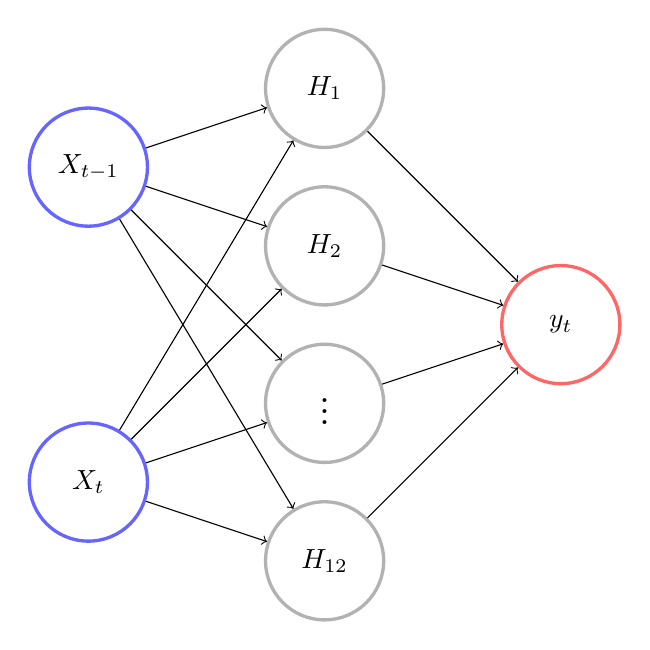
\begin{tikzpicture}[
            neuron/.style={circle, very thick, minimum size=15mm},
            input/.style={draw=blue!60},
            hidden/.style={draw=gray!60},
            output/.style={draw=red!60},]

        % Nodes entrada
        \node[neuron, input]  (entrada1)   at (0, 5cm)   {$X_{t-1}$};
        \node[neuron, input]  (entrada2)   at (0, 1cm)   {$X_{t}$};

        % Nodes escondidos
        \node[neuron, hidden] (escondido1) at (3cm, 6cm) {$H_1$};
        \node[neuron, hidden] (escondido2) at (3cm, 4cm) {$H_2$};
        \node[neuron, hidden] (escondido3) at (3cm, 2cm) {$\LARGE{\vdots}$};
        \node[neuron, hidden] (escondido4) at (3cm, 0)   {$H_{12}$};

        % Nodes Saída
        \node[neuron, output] (saida)      at (6cm, 3cm) {$y_t$};

        \foreach \dest in {1,...,4}
            \path[->] (entrada1) edge (escondido\dest);

        \foreach \dest in {1,...,4}
            \path[->] (entrada2) edge (escondido\dest);

        \foreach \dest in {1,...,4}
            \path[->] (escondido\dest) edge (saida);
    \end{tikzpicture}
    \source{Elaborado pelo autor}
\end{figure}

\chapter{Resultados}\label{chap:result}

\chapter{Conclusões}\label{chap:concl}

\section{Trabalhos futuros}

\postextual

\bibliography{referencias}

\end{document}
